\chapter{轮轴}
\noindent
\begin{figure}[htbp]
\centering
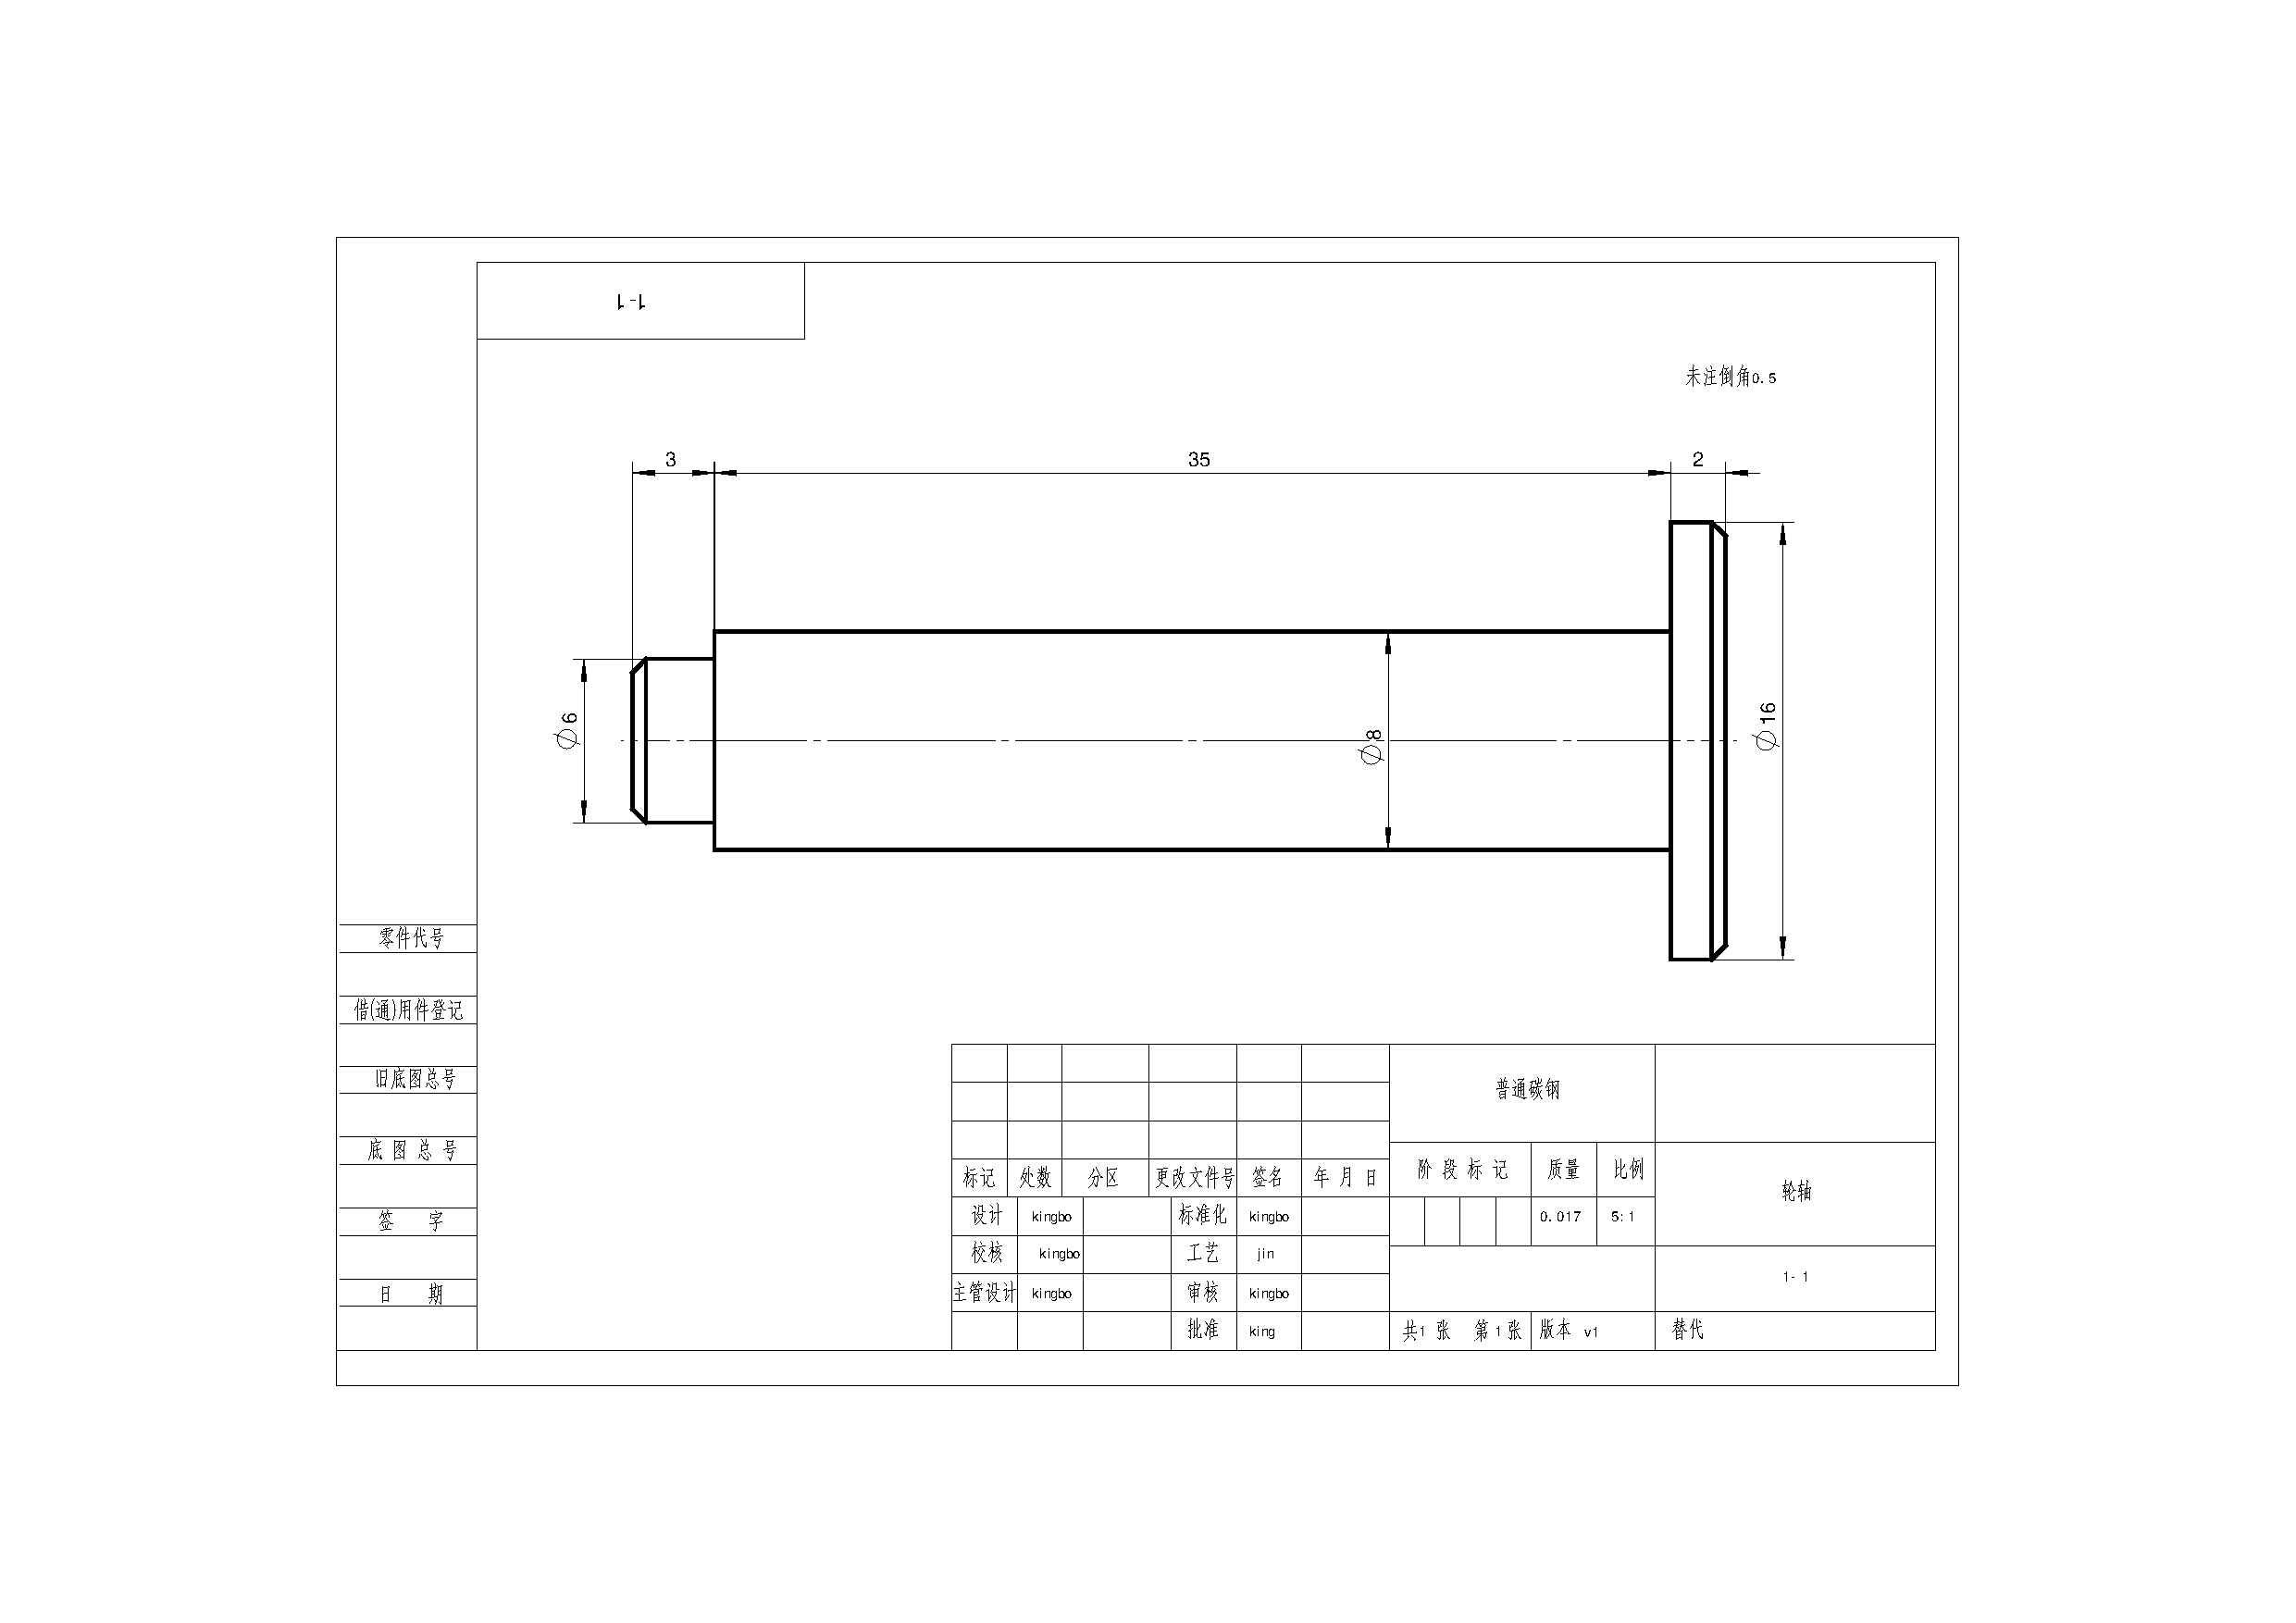
\includegraphics[scale=0.45]{xiaolunzhou.pdf}
\caption{轮轴零件图}\label{fig:xiaolunzhou}
\end{figure}

本简的目标是用AutoCAD制作图\ref{fig:xiaolunzhou}所示轴零件的三维模型,并用布局空间生成该三维模型的主视图,以验证模型的正确性,使学习者进一步理解三维模型与工程零件图之间的关系。因此,本章将讲述以下内容:
\begin{itemize}
	\item 轴零件三维模型的构建
	\item 并集操作
	\item 视图的生成
	\item 图幅和比例的标准
\end{itemize}

\endinput